\documentclass[10pt,bibliography=totocnumbered,listof=totocnumbered, footsepline, headsepline]{scrreprt}
\usepackage[a4paper,top=2.5cm,left=2.5cm,bottom=2cm,right=2cm]{geometry}
\usepackage[english]{babel}
\usepackage[utf8]{inputenc}
\usepackage{amsmath}
\usepackage{mathtools}
\usepackage{amsfonts}
\usepackage{amssymb}
\usepackage{amstext}
\usepackage{graphicx}
\usepackage{tabularx}
\usepackage{setspace}
\usepackage[right]{eurosym}
\usepackage{subfig}
\usepackage[usenames,dvipsnames]{color}
\usepackage{colortbl}
\usepackage{array}
\usepackage{parskip}
\usepackage[right]{eurosym}
\usepackage[pdfpagelabels=true]{hyperref}
\usepackage{listings}
\usepackage[automark]{scrlayer-scrpage}
\usepackage{multicol}
\usepackage{float}
\usepackage{enumerate}
\usepackage{pgfplots}
\usepackage{xcolor}
\usepackage{todonotes}
\usepackage{fontawesome}
\usepackage{pdfpages}

\lstset{ %
	backgroundcolor=\color{white},   % choose the background color
	basicstyle=\footnotesize,        % size of fonts used for the code
	breaklines=true,                 % automatic line breaking only at whitespace
	captionpos=b,                    % sets the caption-position to bottom
	commentstyle=\color{ForestGreen},    % comment style
	escapeinside={\%*}{*)},          % if you want to add LaTeX within your code
	keywordstyle=\color{blue},       % keyword style
	stringstyle=\color{BurntOrange},     % string literal style
}

\definecolor{codegreen}{rgb}{0,0.6,0}
\lstdefinestyle{mystyle}{
    backgroundcolor=\color{black},
    basicstyle=\ttfamily\footnotesize\color{codegreen},
}

% Header Footer
\pagestyle{scrheadings}
\automark[section]{chapter}
\clearscrheadfoot
\ihead[]{TDDI08 and TDTS07 - Embedded Systems Design}
\ohead[]{Design space exploration with MPARM}
\ifoot[]{Simon Burkhardt (simbu448), Jule Enninghorst (julen905)}
\ofoot[]{\thepage}
\addtolength{\footskip}{-4ex}
% Section Deapth
\setcounter{secnumdepth}{4}

%\setcounter{section}{2}
\renewcommand{\thesection}{Assignment \arabic{section}:}
\renewcommand\thefigure{\arabic{figure}}

\renewcommand{\arraystretch}{1.2}


\begin{document}

\title{TDTS07/TDDI08: lab 3 - MPARM}
\author{Simon Burkhardt (simbu448)\\ Jule Eninghorst (julen905)}
\maketitle

\section{Design-Space Exploration for Energy Minimization}

The goal of this task is to minimize the \textbf{energy consumption} of a single CPU task by exploring different configurations of cache type/size and CPU frequency.

\paragraph*{Steps to simulate} 
The following commands are used to execute this lab and reproduce the results presented:

\texttt{source /courses/TDTS07/sw/mparm/go\_mparm\_bash.sh} \\
\texttt{cd <mparm workspace>/benches/gsm-good/single-newmparm/gsm-1.0-pl10-one-task-mparm} \\
\texttt{make -f Makefile.mparm} \\
\texttt{cd bin} \\
\texttt{mpsim.x -cn -w --ds=x --dt=x --is=x --it=x -F x,y} \\

where:

\begin{itemize}
    \item \texttt{-cn} where n is number of CPUs
    \item \texttt{--ds} D-cache size ($2^s$ bytes)
    \item \texttt{--dt} D-cache type (n-way associative)
    \item \texttt{--is} I-cache size ($2^s$ bytes)
    \item \texttt{--it} I-cache type (n-way associative)
    \item \texttt{-F x,y} sets the frequency of CPU Nr. x to $\frac{1}{y}^{th}$ of the system frequency
\end{itemize}

The options unified cache (instead of separate D- and I-cache) and fully associative (instead of n-way) are not available.

\textbf{Command example for one simulation:}\\
\texttt{mpsim.x -c1 -w -F 0,1 --ds=10 --dt=4 --is=10 --it=4 > /dev/null \&\& grep "Total" stats.txt}

\paragraph*{Results}
As shown in Fig. \ref{fig:mparm_1_cache} the reference implementation at maximum CPU frequency uses $45.03\mu$J. 
We first introduce data cache (D) and instruction cache (I) independently to explore, which option could potentially bring the most improvement in energy consumption.
Tests 2 - 6 show an increase in energy consumption with growing data cache size.
Tests 7 - 11 display a great influence on the energy consumption.
The best cache size here seems to be a small one with $2^{10}$ or less bytes.
Adding some D-cache to this I-cache slightly improves the energy (Test Nr. 12).
Next, we reduce the CPU frequency to further improve the efficiency.
Test Nr. 20 uses only $\frac{1}{4}{th}$ of the original CPU frequency which results in an energy consumption of only $17.93\mu$J. This is an improvement of 60\% compared to the un-optimized case at 200 MHz!

\begin{figure}[H]
	\centerline{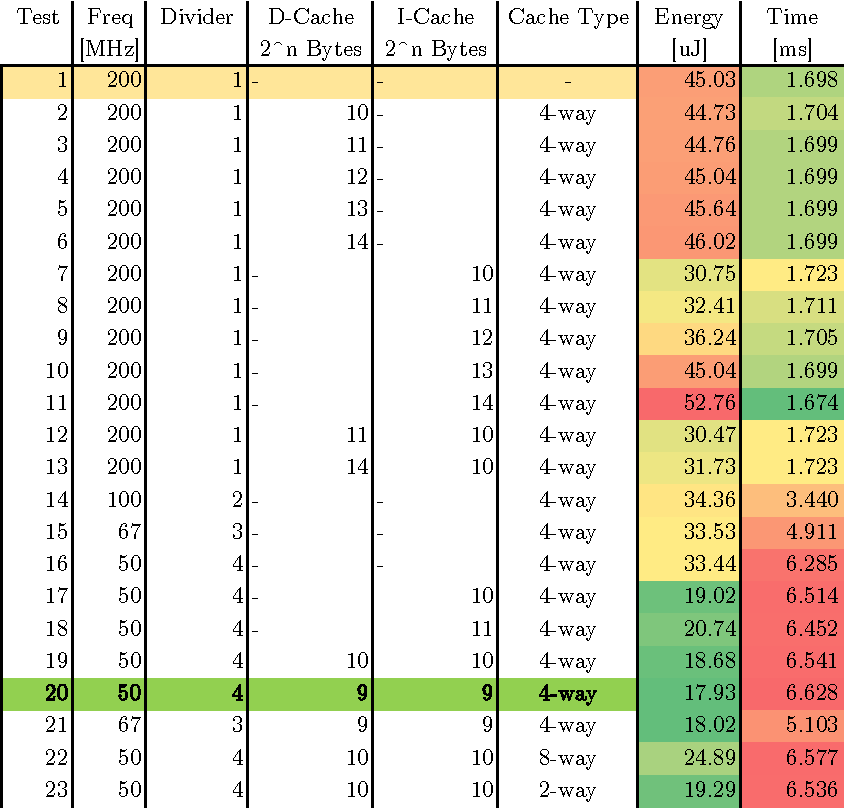
\includegraphics[width=34pc]{mparm_1_cache.pdf}}
	\caption{Explored design space for the GSM one-task exercise where test Nr. 20 results in the lowest consumed energy of 17.93$\mu$J}
	\label{fig:mparm_1_cache}
\end{figure}

\section{Shared Memory vs. Distributed Message Passing}

The goal of this task is to explore how different inter processor communication mechanisms for a multi-core task influence \textbf{BUS usage} as well as energy and execution time. There are a total of 3 CPU cores which can be clocked independently, each at an integer fraction of the $200$ MHz system clock.

\paragraph*{Steps to simulate} 
The following commands are used to execute this lab and reproduce the results presented:

\texttt{source /courses/TDTS07/sw/mparm/go\_mparm\_bash.sh} \\
\texttt{cd benches/gsm-mparm-multiproc-map1} \\
or \\
\texttt{cd benches/gsm-mparm-shared-map1} \\
\texttt{make -f Makefile.mparm} \\
\texttt{cd bin} \\
\texttt{mpsim.x -c3 -C -w -F0,x -F1,y -F2,z} \\

\textbf{Command example for one simulation} \\
\texttt{mpsim.x -c3 -w -C -F0,1 -F1,1 -F2,1 > /dev/null} \\
\texttt{grep "Total" stats.txt} for energy consumption \\
\texttt{grep "\% of" stats.txt} for bus statistics \\

\paragraph*{Results}
The results of the experiment are displayed in the table in Fig. \ref{fig:mparm_2_com}.
The first 2 experiments compare the two different inter-core communication styles.
According to the simulation, the shared memory approach reduces the bus busyness by approximately 11 percent-points but drastically increases energy consumption and execution time.

The experiments 3 - 5 show that the bus usage is naturally reduced, if all the CPU's are running with a slower clock. This makes sense since the bus continues running at the 200 MHz of the reference system.
Therefore, if bus usage is the only concern, one could just lower the CPU frequency of all cores and in turn sacrifice execution time.
Experiments 6 - 8 explore what happens if only a single core is slowed down.

% @todo: Jule. is this all correct? bus at 200 MHz etc...


\begin{figure}[H]
	\centerline{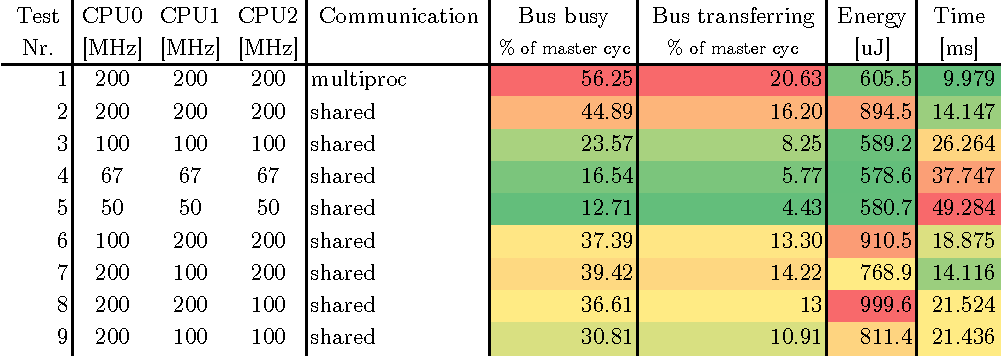
\includegraphics[width=34pc]{mparm_2_com.pdf}}
	\caption{Explored design space for the GSM one-task exercise where test Nr. 20 results in the lowest consumed energy of 17.93$\mu$J}
	\label{fig:mparm_2_com}
\end{figure}


\section{Mapping/Scheduling}

This exercise requires a manual reschedule of a given list of tasks with data dependencies.
Fig. \ref{fig:CPU_Schedule} shows the original schedule alongside the two proposed new schedules.
In both cases, the execution time (SL) can be cut down by 10ms to 35ms which is a 22\% speed improvement.

    \begin{figure*}[h]
    	\centerline{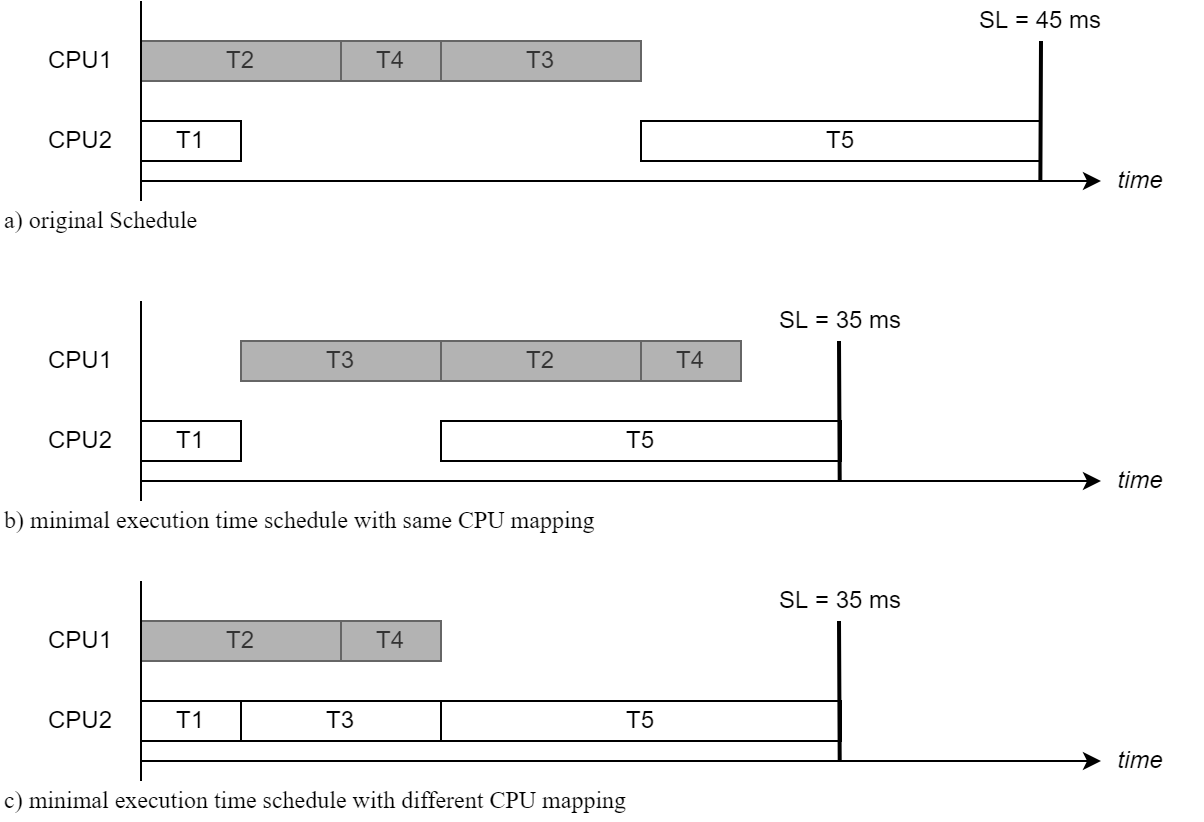
\includegraphics[width=34pc]{CPU_Schedules.png}}
    	\caption{Various task mappings}
    	\label{fig:CPU_Schedule}
    \end{figure*}    

\end{document}
